\documentclass{article}
\usepackage[utf8]{inputenc}

\usepackage{graphicx}
\usepackage[2cm, right=2cm,top=2cm,bottom=2cm]{geometry}

\title{Microprocessor and Assembly Language Lab 03}
\author{Kazi Shadman Sakib, FH-97}
\date{February 10, 2022}

\begin{document}

\maketitle

\section{Task i: Peripheral Clock Configuration}
The RCC peripheral is used to control the internal peripherals, as well as the reset signals and clock distribution. Over the last half-decade, dramatically lowering current draw has been a goal for most microcontroller manufacturers. One of the techniques used to achieve this is to switch off on-chip peripherals by removing access to their master clocks. On the STM32 devices, these clocks are known as the hardware and peripheral clocks and are controlled by the RCC (Reset and Clock Control) group of registers. Since there are more than 32 on chip peripherals, there are actually two registers used to switch on a clock: RCC\textunderscore AHB1 ENR and RCC\textunderscore AHB2ENR for the Hardware clock, APB for the Peripheral clock. The clock is controlled by set/reset registers, so to turn a system on you set a bit in the ENR register, and to turn that same peripheral off you set the bit in the corresponding RCC\textunderscore AHBxRSTR register.

\subsection{Listing out all the clock register of Nucleo-STM32F446RE development board and their respective purpose:}

\textbf{RCC clock control register (RCC\textunderscore CR):} Purpose: Clock control register.\newline\newline
\textbf{RCC PLL configuration register (RCC\textunderscore PLLCFGR)):} Purpose: PLL Configuration register.\newline\newline
\textbf{RCC clock configuration register (RCC\textunderscore CFGR):} Purpose: Clock Configuration register.\newline\newline
\textbf{RCC clock interrupt register (RCC\textunderscore CIR):} Purpose: Clock interrupt register.\newline\newline
\textbf{RCC AHB1 peripheral reset register (RCC\textunderscore AHB1RSTR):} Purpose: AHB1 peripheral reset register.\newline\newline
\textbf{RCC AHB2 peripheral reset register (RCC\textunderscore AHB2RSTR):} Purpose: AHB2 peripheral reset register.\newline\newline
\textbf{RCC AHB3 peripheral reset register (RCC\textunderscore AHB3RSTR):} Purpose: AHB3 peripheral reset register.\newline\newline
\textbf{RCC APB1 peripheral reset register (RCC\textunderscore APB1RSTR):} Purpose: APB1 peripheral reset register.\newline\newline
\textbf{RCC APB2 peripheral reset register (RCC\textunderscore APB2RSTR):} Purpose: APB2 peripheral reset register.\newline\newline
\textbf{RCC AHB1 peripheral clock enable register (RCC\textunderscore AHB1ENR):} Purpose: AHB1 peripheral enable register\newline\newline
\textbf{RCC AHB2 peripheral clock enable register (RCC\textunderscore AHB2ENR):} Purpose: AHB2 peripheral enable register.\newline\newline
\textbf{RCC AHB3 peripheral clock enable register (RCC\textunderscore AHB3ENR):} Purpose: AHB3 peripheral enable register.\newline\newline
\textbf{RCC APB1 peripheral clock enable register (RCC\textunderscore APB1ENR):} Purpose: APB1 peripheral enable register\newline\newline
\textbf{RCC APB2 peripheral clock enable register (RCC\textunderscore APB2ENR):} Purpose: APB2 peripheral enable register.\newline\newline
\textbf{RCC AHB1 peripheral clock enable in low power mode register (RCC\textunderscore AHB1LPENR):} Purpose: AHB1 peripheral enable in low power register.\newline\newline
\textbf{RCC AHB2 peripheral clock enable in low power mode register (RCC\textunderscore AHB2LPENR):} Purpose: AHB2 peripheral enable in low power register.\newline\newline
\textbf{RCC AHB3 peripheral clock enable in low power mode register (RCC\textunderscore AHB3LPENR):} Purpose: AHB3 peripheral enable in low power register.\newline\newline
\textbf{RCC APB1 peripheral clock enable in low power mode register (RCC\textunderscore APB1LPENR):} Purpose: APB1 peripheral enable in low power register.\newline\newline
\textbf{RCC APB2 peripheral clock enabled in low power mode register (RCC\textunderscore APB2LPENR):} Purpose: APB2 peripheral enable in low power register.\newline\newline
\textbf{RCC Backup domain control register (RCC\textunderscore BDCR):} Purpose: Backup Domain control register.\newline\newline
\textbf{RCC clock control & status register (RCC\textunderscore CSR):} Purpose: Clock control and status register.\newline\newline
\textbf{RCC spread spectrum clock generation register (RCC\textunderscore SSCGR):} Purpose: Spread spectrum clock generation register.\newline\newline
\textbf{RCC PLLI2S configuration register (RCC\textunderscore PLLI2SCFGR):} Purpose: PLLI2S configuration register.\newline\newline
\textbf{RCC PLL configuration register (RCC\textunderscore PLLSAICFGR):} Purpose: PLLSAI configuration register.\newline\newline
\textbf{RCC dedicated clock configuration register (RCC\textunderscore DCKCFGR):} Purpose: Dedicated clocks configuration register.\newline\newline
\textbf{RCC clocks gated enable register (CKGATENR):} Purpose: RCC clocks gated enable register.\newline\newline
\textbf{RCC dedicated clocks configuration register 2 (DCKCFGR2):} Purpose: RCC Dedicated Clocks Configuration Register 2.\newline\newline


\subsection{Listing the memory address of the clock registers:}

\textbf{RCC clock control register (RCC\textunderscore CR):} Address offset: 0x00\newline\newline
\textbf{RCC PLL configuration register (RCC\textunderscore PLLCFGR)):} Address offset: 0x04\newline\newline
\textbf{RCC clock configuration register (RCC\textunderscore CFGR):} Address offset: 0x08\newline\newline
\textbf{RCC clock interrupt register (RCC\textunderscore CIR):} Address offset: 0x0C\newline\newline
\textbf{RCC AHB1 peripheral reset register (RCC\textunderscore AHB1RSTR):} Address offset: 0x10\newline\newline
\textbf{RCC AHB2 peripheral reset register (RCC\textunderscore AHB2RSTR):} Address offset: 0x14\newline\newline
\textbf{RCC AHB3 peripheral reset register (RCC\textunderscore AHB3RSTR):} Address offset: 0x18\newline\newline
\textbf{RCC APB1 peripheral reset register (RCC\textunderscore APB1RSTR):} Address offset: 0x20\newline\newline
\textbf{RCC APB2 peripheral reset register (RCC\textunderscore APB2RSTR):} Address offset: 0x24\newline\newline
\textbf{RCC AHB1 peripheral clock enable register (RCC\textunderscore AHB1ENR):} Address offset: 0x30\newline\newline
\textbf{RCC AHB2 peripheral clock enable register (RCC\textunderscore AHB2ENR):} Address offset: 0x34\newline\newline
\textbf{RCC AHB3 peripheral clock enable register (RCC\textunderscore AHB3ENR):} Address offset: 0x38\newline\newline
\textbf{RCC APB1 peripheral clock enable register (RCC\textunderscore APB1ENR):} Address offset: 0x40\newline\newline
\textbf{RCC APB2 peripheral clock enable register (RCC\textunderscore APB2ENR):} Address offset: 0x44\newline\newline
\textbf{RCC AHB1 peripheral clock enable in low power mode register (RCC\textunderscore AHB1LPENR):} Address offset: 0x50\newline\newline
\textbf{RCC AHB2 peripheral clock enable in low power mode register (RCC\textunderscore AHB2LPENR):} Address offset: 0x54\newline\newline
\textbf{RCC AHB3 peripheral clock enable in low power mode register (RCC\textunderscore AHB3LPENR):} Address offset: 0x58\newline\newline
\textbf{RCC APB1 peripheral clock enable in low power mode register (RCC\textunderscore APB1LPENR):} Address offset: 0x60\newline\newline
\textbf{RCC APB2 peripheral clock enabled in low power mode register (RCC\textunderscore APB2LPENR):} Address offset: 0x64\newline\newline
\textbf{RCC Backup domain control register (RCC\textunderscore BDCR):} Address offset: 0x70\newline\newline
\textbf{RCC clock control & status register (RCC\textunderscore CSR):} Address offset: 0x74\newline\newline
\textbf{RCC spread spectrum clock generation register (RCC\textunderscore SSCGR):} Address offset: 0x80\newline\newline
\textbf{RCC PLLI2S configuration register (RCC\textunderscore PLLI2SCFGR):} Address offset: 0x84\newline\newline
\textbf{RCC PLL configuration register (RCC\textunderscore PLLSAICFGR):} Address offset: 0x88\newline\newline
\textbf{RCC dedicated clock configuration register (RCC\textunderscore DCKCFGR):} Address offset: 0x8C\newline\newline
\textbf{RCC clocks gated enable register (CKGATENR):} Address offset: 0x90\newline\newline
\textbf{RCC dedicated clocks configuration register 2 (DCKCFGR2):} Address offset: 0x94\newline\newline

\section{Task ii: General Purpose Input/ Output Registers}

Each General-Purpose I/O port has four 32-bit configuration registers (GPIOx \textunderscore MODER, GPIOx\textunderscore OTYPER, GPIOx\textunderscore OSPEEDR and GPIOx\textunderscore PUPDR), two 32-bit data registers (GPIOx\textunderscore IDR and GPIOx\textunderscore ODR), a 32-bit set/reset register (GPIOx\textunderscore BSRR), a 32-bit locking register (GPIOx\textunderscore LCKR) and two 32-bit alternate function selection register (GPIOx\textunderscore AFRH and GPIOx\textunderscore AFRL).

\subsection{Listing out all the GPIO register of Nucleo-STM32F446RE development board and their respective purpose:}

\textbf{Mode Register (GPIOx\textunderscore MODER): } The GPIOx\textunderscore MODER register is a 32-bit memory-mapped control register to configure upto 16 I/Os. The GPIOx\textunderscore MODER register is used to select the I/O direction (input, output, AF, analog). The configuration length of each port mode register is 2 bits.\newline\newline
Bits 2y:2y+1: \newline\newline
These configuration bits are written by software to configure the I/O direction mode: \newline\newline
00: Input (reset state) \newline\newline
01: General purpose output mode \newline\newline
10: Alternate function mode \newline\newline
11: Analog mode \newline\newline

Very commonly used modes are input mode, general purpose output mode and alternate function mode. ADC or DAC uses Analog mode. Also, whenever a microcontroller undergoes reset all the pins of different GPIO ports will be by default in the input state. \newline\newline

\textbf{Output Type Register (GPIOx\textunderscore OTYPER):} The GPIOx\textunderscore OTYPER register is a 32-bit memory-mapped control register to configure upto 16 I/Os. The GPIOx\textunderscore OTYPER register is used to select the output type-\newline\newline

\textbf{a) Push-Pull mode: }In push-pull mode “0” in the Output data register activates the N-MOS whereas a “1” in the Output data register activates the P-MOS. The data present on the I/O pin is sampled into the input data register over every AHB1 clock cycle. Read access to the input data register gets the I/O state. Read access to the output data register gets the last written value. To set GPIO output type register in push-pull mode, in GPIO\textunderscore OTYPER register bit is set to “0”.\newline\newline

\textbf{b) Open Drain mode: }In Open-drain configuration, PMOS doesn’t exist, and two
output possibilities are high or floating. A “0” in the Output data register activates the N-MOS and the I/O pin driven to the ground. Whereas “1” in the Output data register leaves the port in Hi-Z (the P-MOS is never activated), so I/O state is not defined. To solve this issue either activate an internal pull-up resistor or give an external pull-up resistor. So, once a pull-up resistor is activated, the I/O pin gets its state to VDD. To set GPIO output type register in open-drain mode, in GPIO\textunderscore OTYPER register bit is set to “1”. \newline\newline
Bits 31:16 are Reserved. Only Bits 15:0 are used.\newline\newline
The configuration bits are written by software to configure the output type of the I/O port.\newline\newline
0: Output Push-Pull (reset state)\newline\newline
1: Output Open-Drain\newline\newline

\textbf{Speed Register (GPIOx\textunderscore xOSPEEDR): } The GPIOx\textunderscore OSPEEDR register is a 32-bit memory-mapped control register to configure upto 16 I/Os. The GPIOx\textunderscore OSPEED register is used to select the speed (the I/O speed pins are directly connected to the corresponding GPIOx\textunderscore OSPEEDR register bits whatever the I/O direction). It is only applicable when the GPIO pin is in output mode. By using the GPIO output speed register, one can configure the GPIO transitions from high to low and low to high, which means the slew rate of a pin can be controlled by GPIO output speed register.\newline\newline
Bits 2y:2y+1:\newline\newline
These bits are written by software to configure the I/O output speed.\newline\newline
00: Low speed\newline\newline
01: Medium speed\newline\newline
10: Fast speed\newline\newline
11: High speed\newline\newline

\textbf{Pull-UP / Pull-Down Register (GPIOx\textunderscore PUPDR): } The GPIOx\textunderscore PUPDR register is a 32-bit memory-mapped control register to configure upto 16 I/Os. The GPIOx\textunderscore PUPDR register is used to select the Pull-Up / Pull-Down whatever the I/O direction. GPIO Pull-Up and Pull-Down registers are used to control the internal or external Pull-Up and Pull-Down registers.
Bits 2y:2y+1:\newline\newline
These bits are written by software to configure the I/O pull-up or pull-down.\newline\newline
00: No pull-up, pull-down\newline\newline
01: Pull-Up\newline\newline
10: Pull-Down\newline\newline
11: Reserved\newline\newline
\textbf{GPIO port Bit Set and Reset Register (GPIOx\textunderscore BSRR): }
The Bit Set and Reset register (GPIOx\textunderscore BSRR) is a 32-bit register which allows the application to set and reset each individual bit in the output data register (GPIOx\textunderscore ODR). The purpose of the GPIOx\textunderscore BSRR register is to allow atomic read/modify accesses to any of the GPIO registers. In this way, there is no risk of an IRQ occurring between the read and the modify access. The GPIOx\textunderscore BSRR register provides a way of performing atomic bitwise handling. It is possible to modify one or more bits in a single atomic AHB1 write access. This register consists of two write-only bit masks, each 16-bit wide. The high half- 16 bits to 31 is the reset mask. Writing a 1 to any of these bits clear bit N-16 in the GPIO\textunderscore ODR. The low half - bits 0 to 15 is the set mask. Writing a 1 to any of these bits sets the corresponding bit in the GPIO\textunderscore ODR.\newline\newline

Bits 31:16 BRy: Port x reset bit y\newline\newline
These bits are write-only and can be accessed in word, half-word or byte mode. A read to these bits return the value 0x0000.\newline\newline
0: No action on the corresponding ODRx bit\newline\newline
1: Resets the corresponding ODRx bit\newline\newline
Bits 15:0 BSy: Post x set bit y\newline\newline
These bits are write-only and can be accessed in word, half-word or byte mode. A read to these bits return the value 0x0000.\newline\newline
0: No action on the corresponding ODRx bit\newline\newline
1: Sets the corresponding ODRx bit\newline\newline

\textbf{Alternate Function (AF): } Two registers are provided to select one out of the sixteen Alternate Function inputs/outputs available for each I/O. With these registers, one can connect an alternate function to some other pin as required by an application. This means that a number of possible peripheral functions are multiplexed on each GPIO using these two alternate registers-\newline\newline
\textbf{a) GPIO Alternate Function Low Register (GPIOx\textunderscore AFRL): } GPIOx\textunderscore AFRL contains the multiplexer settings for port bits 0 to 7.\newline\newline
Bits 31:0 Alternate function selection for port x bit y\newline\newline
These bits are written by software to configure alternate functions I/Os.\newline\newline
AFRLy selection:\newline\newline
0000: AF0 1000: AF8\newline\newline
0001: AF1 1001: AF9\newline\newline
0010: AF2 1010: AF10\newline\newline
0011: AF3 1011: AF11\newline\newline
0100: AF4 1100: AF12\newline\newline
0101: AF5 1101: AF13\newline\newline
0110: AF6 1110: AF14\newline\newline
0111: AF7 1111: AF15\newline\newline

\textbf{b) GPIO Alternate Function High Register (GPIOx\textunderscore AFRH):} GPIOx\textunderscore AFRH contains the multiplexer settings for port bits 8 to 15.\newline\newline
Bits 31:0 Alternate function selection for port x bit y\newline\newline
These bits are written by software to configure alternate functions I/Os. AFRHy selection:\newline\newline
0000: AF0 1000: AF8\newline\newline
0001: AF1 1001: AF9\newline\newline
0010: AF2 1010: AF10\newline\newline
0011: AF3 1011: AF11\newline\newline
0100: AF4 1100: AF12\newline\newline
0101: AF5 1101: AF13\newline\newline
0110: AF6 1110: AF14\newline\newline
0111: AF7 1111: AF15\newline\newline
The application can thus select any one of the possible functions for each I/O. The AF selection signal being common to the alternate function input and alternate function output, a single channel is selected for the alternate function input/output of one I/O.\newline\newline
\textbf{Some more functions and roles of related Registers with GPIO Port and Pins:\newline\newline}
\textbf{Input Data Register (GPIOx\textunderscore IDR): } The input data register (GPIOx\textunderscore IDR) is a 16-bit memory-mapped data register. The input data register (GPIOx\textunderscore IDR) captures the data present on the I/O pin at every AHB1 clock cycle. The data input through the I/O are stored into the input data register (GPIOx\textunderscore IDR), a read-only register. Here only Bits 15:0 are used and 31:16 bits are reserved.\newline\newline
\textbf{Output Data Register (GPIOx\textunderscore ODR): }
The output data register (GPIOx\textunderscore ODR) is a 16-bit memory-mapped data register. When the pin is configured as output, the value written to the output data register (GPIOx\textunderscore ODR) is output on the I/O pin. It is possible to use the output driver in push-pull mode or open-drain mode (only the N-MOS is activated when 0 is output). GPIOx\textunderscore ODR stores the data to be output, it is read/write accessible. Here only 16-bits are used in this register. So, 16 to 31 are reserved, and the 0th-bit position will control the I/O pin 0.\newline\newline

\textbf{Configuration Lock Register (GPIOx\textunderscore LCKR): } It is possible to freeze the GPIO control registers by applying a specific write sequence to the GPIOx\textunderscore LCKR register. The frozen registers are GPIOx\textunderscore MODER, GPIOx\textunderscore OTYPER,GPIOx\textunderscore OSPEEDR,GPIOx\textunderscore PUPDR,GPIOx\textunderscore AFRL, GPIOx\textunderscore AFRH.\newline\newline
\textbf{Analog Switch Control Register (GPIOx\textunderscore ASCR): } GPIOx\textunderscore ASCR register helps to control analog interconnection between an I/O pin and ADC input.

\subsection{Listing the memory address of the GPIO registers: }\newline\newline
\textbf{Mode Register (GPIOxMODER): } Address offset: 0x00\newline\newline
\textbf{Output Type Register (GPIOxOTYPER): } Address offset: 0x04\newline\newline
\textbf{Speed  Register  (GPIOxxOSPEEDR): } Address offset: 0x08\newline\newline
\textbf{Pull-UP  /  Pull-Down  Register  (GPIOxPUPDR): } Address offset: 0x0C\newline\newline
\textbf{GPIO port Bit Set and Reset Register (GPIOxBSRR): } Address offset: 0x18\newline\newline
\textbf{GPIO  Alternate  Function  Low  Register  (GPIOxAFRL): } Address offset: 0x20\newline\newline
\textbf{GPIO Alternate Function High Register (GPIOxAFRH): } Address offset: 0x24\newline\newline
\textbf{Input Data Register (GPIOxIDR): } Address offset: 0x10\newline\newline
\textbf{Output Data Register (GPIOxODR): } Address offset: 0x14\newline\newline
\textbf{Configuration Lock Register (GPIOxLCKR): } Address offset: 0x1C\newline\newline

\section{Task iii} 

\subsection{Detailed Code Explanation}

Allocated two halfword of memory as 0x0032 and 0x0124 in V1 and V2 using the DSD instruction. Then in the main2 identifier Loaded the variable V1 to the register r1 and Loaded the variable V2 to the register r2 using the LDR instruction. AND Operation on r1 and r2 and storing result it in r3 using AND instruction. OR operation on r1 and r2 and storing result it in r4 using ORR instruction. Using the MVN instruction the NOR operation was done on r4 register and saved the result in r5 register. Using the MVN instruction the NAND operation was done on r3 and result was saved in r6 register. XOR operation was done on registers r1 and r2 and then result was stored in r7 register using EOR instruction. And lastly MVN instruction was used to do the XNOR operation on r7 and saved it to r8 register. 

\subsection{Detailed description of the instruction used to design the program.}

LDR: ARM uses a load model for memory access which means that only load (LDR) instruction can access memory and load a value from the memory to the register.\newline\newline
AND:The AND instruction is used for supporting logical expressions by performing bitwise AND operation. The bitwise AND operation returns 1, if the matching bits from both the operands are 1, otherwise it returns 0.\newline\newline
ORR:The OR instruction is used for supporting logical expression by performing bitwise OR operation. The bitwise OR operator returns 1, if the matching bits from either or both operands are one. It returns 0, if both the bits are zero.\newline\newline
MVN:Operation The MVN instruction takes the value of Operand2, performs a bitwise logical NOT operation on the value, and places the result into Rd.\newline\newline
EOR:The EOR instruction performs bitwise Exclusive OR operations on the values in Rn and Operand2.\newline\newline
DCD:DCD is used to "reserve a 32 bit word"\newline\newline

\subsection{Screenshot of Debugger}


\subsubsection{After the Code has been Loaded}

\textbf{For 16 Bit}\newline\newline
\begin{center}
    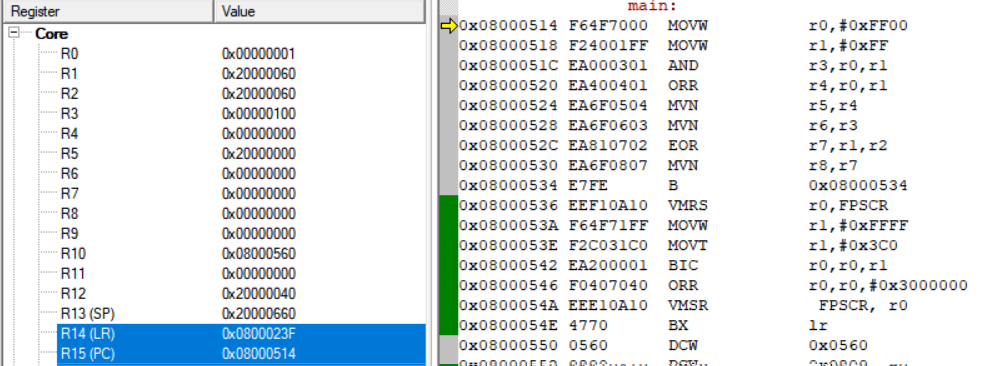
\includegraphics[width=1\textwidth]{16Bit_Before.png}
\end{center}

\textbf{For 32 Bit}\newline\newline
\begin{center}
    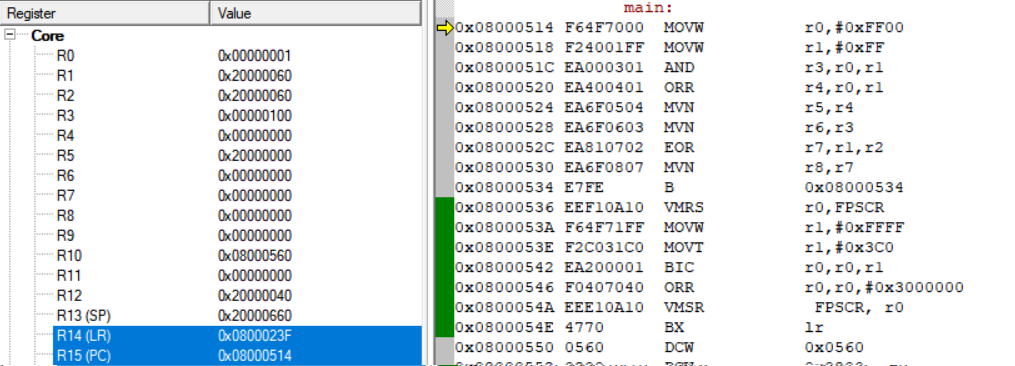
\includegraphics[width=1\textwidth]{32Bit_Before.png}
\end{center}

\subsubsection{After the Code has been Executed}

\textbf{For 16 Bit}\newline\newline
\begin{center}
    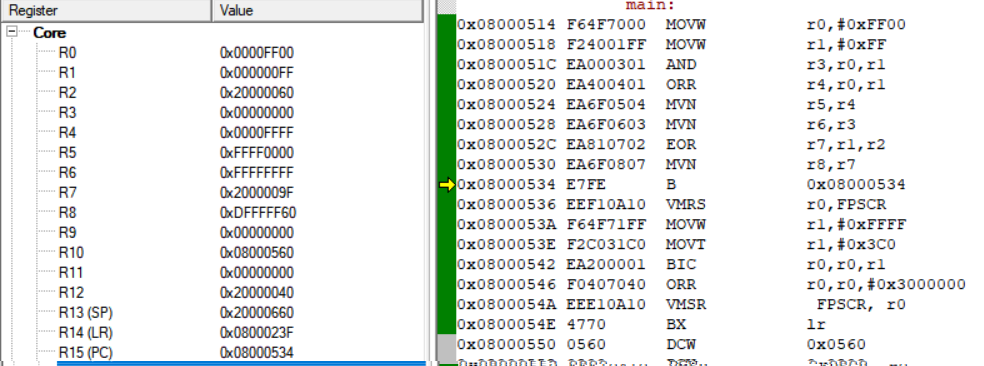
\includegraphics[width=1\textwidth]{16Bit_After.png}
\end{center}\newline\newline

\textbf{For 32 Bit}\newline\newline
\begin{center}
    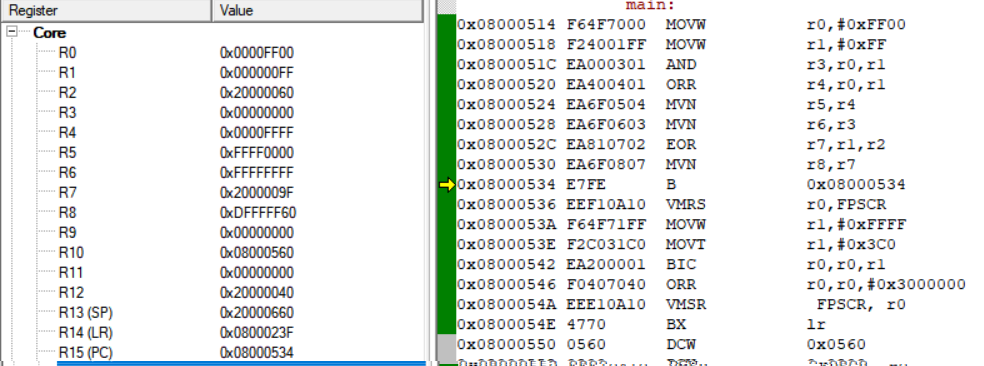
\includegraphics[width=1\textwidth]{16Bit_After.png}
\end{center}

\section{Task iv} 

\subsection{Detailed Code Explanation}

Allocated two halfword of memory as 0x0032 and 0x0124 in V1 and V2 variables. Used the LDR instruction to load the variable V1 in r1 register. LSR instruction was done to use logical shift right operation on r1 by 2 places bits and stored the result in r2. ASR instruction was done to provide the signed value of the contents of a register divided by a power of two and stored it in r3 register. Lastly, used the LSL instruction to logical shift left by 2 places.

\subsection{Detailed description of the instruction used to design the program.}

DCD:DCD is used to "reserve a 32 bit word"\newline\newline
LDR: ARM uses a load model for memory access which means that only load (LDR) instruction can access memory and load a value from the memory to the register.\newline\newline
LSR: LSR is a logical shift right by 0 to 32 places.\newline\newline
ASR:ASR provides the signed value of the contents of a register divided by a power of two. It copies the sign bit into vacated bit positions on the left. Thumb instructions must not use PC or SP.\newline\newline
LSL: LSL is a logical shift left by 0 to 31 places.\newline\newline


\subsection{Screenshot of Debugger}


\subsubsection{After the Code has been Loaded}

\begin{center}
    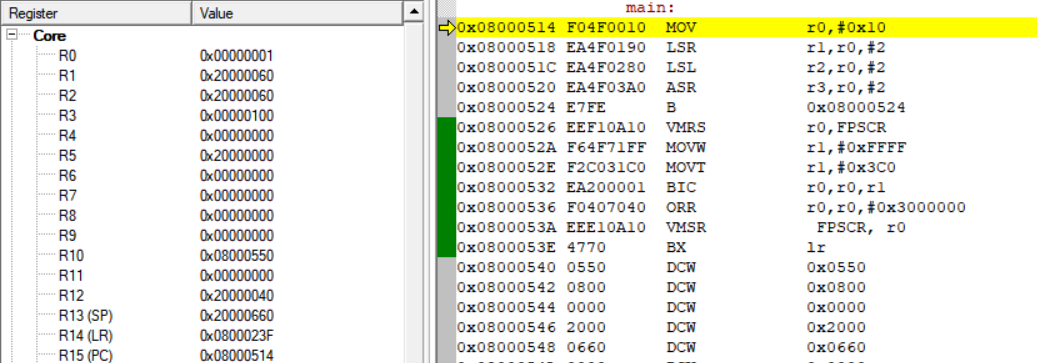
\includegraphics[width=1\textwidth]{Shift_Operation_Before.png}
\end{center}

\subsubsection{After the Code has been Executed}

\begin{center}
    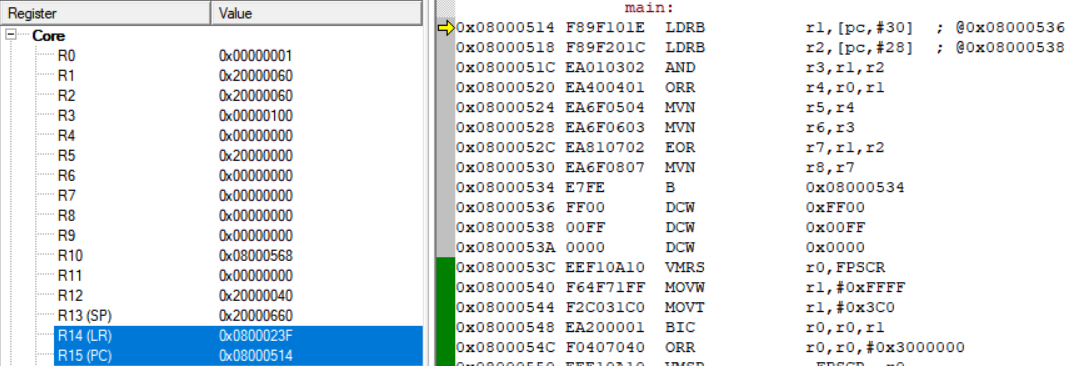
\includegraphics[width=1.3\textwidth]{Shift_Operation_After.png}
\end{center}

\section{Task v} 

\subsection{Detailed Code Explanation}

First, we move the value 0xBBBABABABA to register r1 and 0xEFEFEFEFEF to register r2.\\\\
    Register r2 contains the addition result of values stored in register r0 and r1 and updates a flag register if there is an overflow using the ADDS command. If overflow occurs, we branch to sum\_overflow\\\\
    Register r4 contains the subtraction result of values stored in register r0 and r1 and updates a flag register if there is an overflow using the SUBS command. If overflow occurs, we branch to sub\_overflow.\\\\
    Register r6 contains the multiplication result of values stored in r0 and r1 and sets the value of register r7 to 1 if overflow occurs and branch to label mult\_overflow.
\subsection{Detailed description of the instruction used to design the program.}

DCD:DCD is used to "reserve a 32 bit word"\newline\newline
LDR: ARM uses a load model for memory access which means that only load (LDR) instruction can access memory and load a value from the memory to the register.\newline\newline
MOVT:. In the Thumb instruction set MOVT, instruction moves 16-bit immediate value to top halfword (bits 16 to 31) and the bottom halfword remains unaltered. \newline\newline
ADDS: Addition operation o the registers\newline\newline
SUBS: Subtraction operation o the registers\newline\newline
MUL:This instruction is for multiplying binary data. The MUL (Multiply) instruction handles unsigned data\newline\newline
ADC:The ADC (Add with Carry) instruction adds the values in Rn and Operand2 , together with the carry flag. You can use ADC to synthesize multiword arithmetic.\newline\newline
BCC:BCC (short for "Branch if Carry is Clear") is the mnemonic for a machine language instruction which branches, or "jumps", to the address specified if, and only if the carry flag is clear.\newline\newline
B:The B instruction causes a branch to label.\newline\newline
UMULL:The UMULL instruction interprets the values from Rn and Rm as unsigned integers. It multiplies these integers and places the least significant 32 bits of the result in Rd\newline

\subsection{Status of the status registers after the operation}

\textbf{Status Initial: }\newline\newline

\begin{center}
    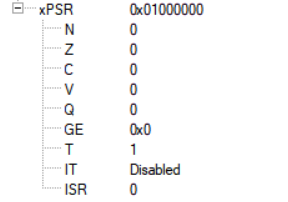
\includegraphics[width=0.4\textwidth]{Status_Initial.png}
\end{center}

\textbf{Status Mid: }\newline\newline

\begin{center}
    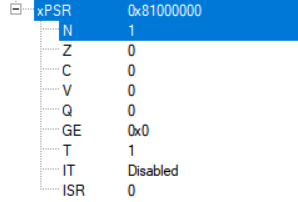
\includegraphics[width=0.4\textwidth]{Status_Mid.png}
\end{center}

\textbf{Status Final: }\newline\newline

\begin{center}
    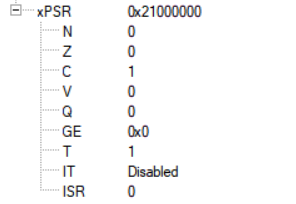
\includegraphics[width=0.4\textwidth]{Status_Final.png}
\end{center}

\subsection{Screenshot of Debugger}


\subsubsection{After the Code has been Loaded}

\textbf{For Arithmetics with Restriction}\newline\newline
\begin{center}
    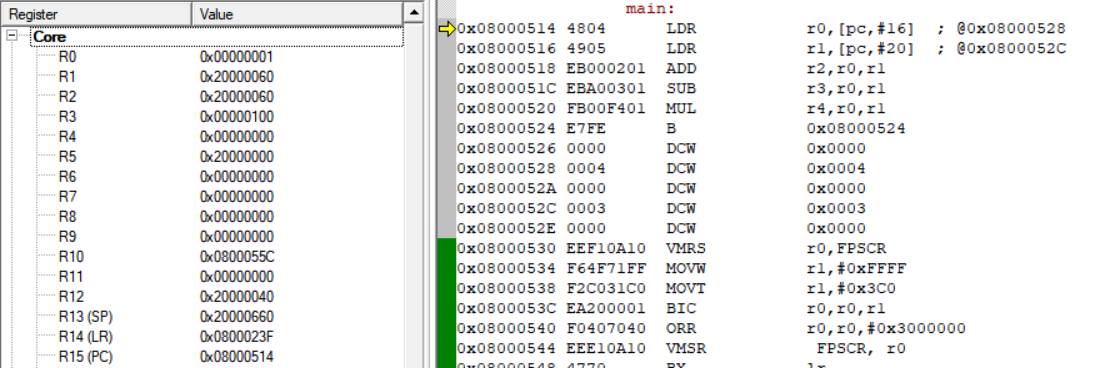
\includegraphics[width=1\textwidth]{Arithmetics_Before.png}
\end{center}

\textbf{For Arithmetics with Overflow handle}\newline\newline
\begin{center}
    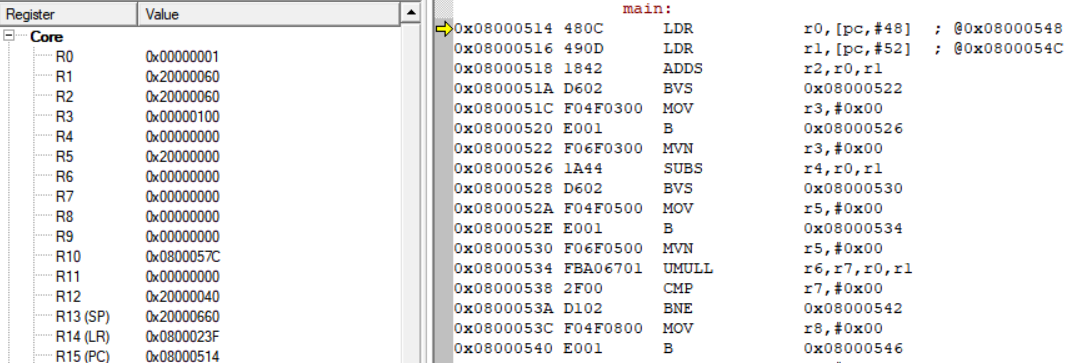
\includegraphics[width=1\textwidth]{Arithmetics_Overflow_Before.png}
\end{center}

\subsubsection{After the Code has been Executed}

\textbf{For Arithmetics with Restriction}\newline\newline
\begin{center}
    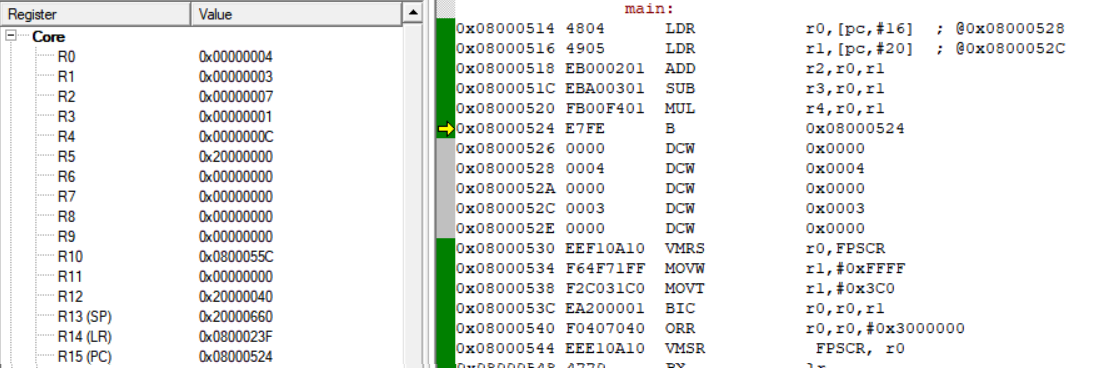
\includegraphics[width=1\textwidth]{Arithmetics_After.png}
\end{center}

\textbf{For Arithmetics with Overflow handle}\newline\newline
\begin{center}
    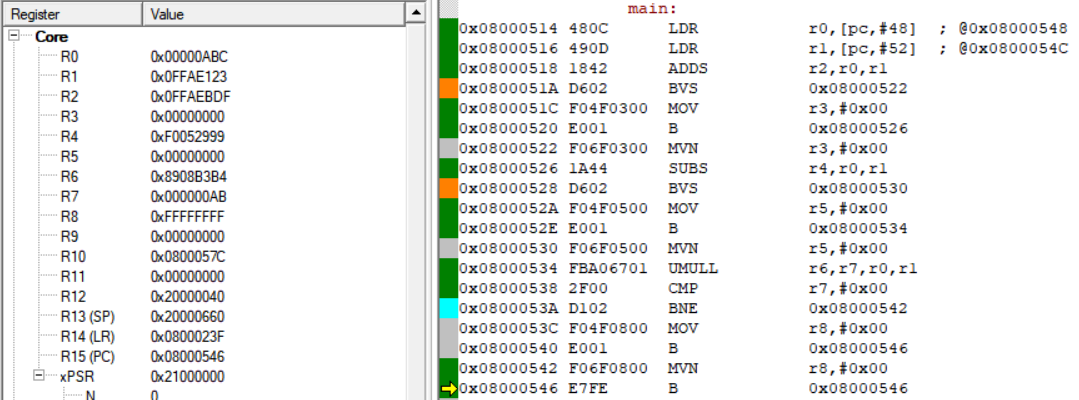
\includegraphics[width=1\textwidth]{Arithmetics_Overflow_After.png}
\end{center}


\end{document}
